\documentclass[10pt]{article}
\usepackage{fontspec}
\setmainfont{Noto Serif CJK SC}
\setsansfont{Noto Sans CJK SC}
\XeTeXlinebreaklocale "zh"
\XeTeXlinebreakskip=0pt plus 1pt
\usepackage[a4paper,margin=20mm]{geometry}
\usepackage{amsmath,amssymb,booktabs,graphicx,microtype,url,xcolor,float}
\usepackage[section]{placeins}
\usepackage[hidelinks]{hyperref}
\usepackage[numbers,sort&compress]{natbib}
\setlength{\emergencystretch}{2em}
\renewcommand{\abstractname}{摘要}
\renewcommand{\refname}{参考文献}
\renewcommand{\figurename}{图}
\renewcommand{\tablename}{表}
\graphicspath{{../../results/figures/}}
\newcommand{\TargetCount}{60}
\newcommand{\ModelCount}{3}
\newcommand{\BlockCount}{180}
\newcommand{\EpisodeCount}{1080}
\newcommand{\MatchedFarRate}{97.8}
\newcommand{\LureNearRate}{10.0}
\newcommand{\BindingRate}{14.4}
\newcommand{\PrimaryEffect}{87.8}
\newcommand{\PrimaryCILow}{82.8}
\newcommand{\PrimaryCIHigh}{93.3}
\newcommand{\MacroEffect}{87.7}
\newcommand{\MacroCILow}{82.7}
\newcommand{\MacroCIHigh}{93.3}
\newcommand{\RandomizationP}{1.00\times 10^{-6}}
\newcommand{\CausalNet}{83.3}
\newcommand{\HarmRate}{0.0}
\newcommand{\HelpfulCount}{150}
\newcommand{\HarmfulCount}{0}


\title{同词不同法：面向可复用 LLM Agent 技能的反事实迁移测试}
\author{匿名作者}
\date{匿名稿，2026 年 9 月}

\begin{document}
\maketitle

\begin{abstract}
Agent 在获得可复用 Skill 后完成新任务，并不能证明成功是由 Skill 引起的：
基础 Agent 可能本来就能完成任务，语义检索也可能选中一个重复目标名词、却
规定错误状态转换的来源。本文提出反事实技能迁移测试（Counterfactual Skill
Transfer Test，CSTT），在同一个原生目标状态上交叉操纵来源技能的程序兼容性
和词面相似度。每个来源都是一条成功的 ALFWorld 训练轨迹，被编译为角色归一
的程序和小型可执行契约。每个目标都从相同状态重置并运行六个条件：无 Skill、
仅绑定、程序匹配的近/远来源，以及程序不匹配的近/远诱饵。仅绑定对照具有
相同的目标落地与搜索守卫，但不接收来源程序，因此可以把执行器帮助与 Skill
因果贡献分开。两个失败的试验机制和最后一次修订完成后，我们冻结源码、来源
分配、三个模型修订、零重叠任务名单、统计检验和决策门槛。确认实验包括
\TargetCount{} 个未参与开发的原生目标、\ModelCount{} 个本地模型家族、
\BlockCount{} 个配对目标--模型块和 \EpisodeCount{} 次执行。程序匹配但
词面最远的来源成功率为 \MatchedFarRate\%，程序错误但词面最近的诱饵为
\LureNearRate\%，配对提高 \PrimaryEffect{} 个百分点（95\% 按目标分层
自助法区间 \PrimaryCILow--\PrimaryCIHigh；按任务聚类的随机化检验
$p=\RandomizationP$）。六任务族等权宏平均提高 \MacroEffect{} 点；相对仅
绑定对照的净因果效应为 \CausalNet{} 点，伤害率为 \HarmRate\%。CSTT 是
评测与贡献归因工具，不是检索算法；本文证据仅支持一个具身文本环境中的实例级
迁移。
\end{abstract}

\noindent\textbf{关键词：}LLM Agent；Agent Skill；技能迁移；反事实评测；
程序兼容性；负迁移

\section{引言}
可复用 Skill 把一次成功的 Agent 经历变为能够在后续任务中检索的持久资产。
近期研究开始抽象实现细节、选择 Skill 粒度、压缩重复经验，并在任务或域之间
适配技能记忆\citep{yu2026polyskill,feng2026breakdown,xu2026compression,
miao2026skilllens,he2026beyond}。这些系统通常报告使用 Skill 后的下游成功率。
该指标有运行价值，却不足以把成功归因给 Skill。

实际部署有两个重要混杂因素。第一，能力更强的基础 Agent 可能在没有任何技能
资产时就能完成目标，把这种执行计作迁移会高估技能库价值。第二，语义检索器
可能偏好共享对象和目标容器、但程序不同的来源。“移动一个对象”和“移动两个
对象”在词面上可以非常接近；加热后放置的来源也可能重复同一对象名，却加入
目标不需要的状态转换。错误来源在单调任务上可能碰巧成功，在其他任务上会
伤害成功率，或者消耗大量交互后才失败。已有全生命周期研究和失败分析说明，
Skill 效用取决于抽取器、消费模型、失配类型和执行上下文
\citep{huang2026consumption,dong2026harmful}。目前缺少的是：在完全相同的原生
状态上，把程序结构和表面词语分离的受控检验。

本文提出 CSTT。对每个目标，测试从真实成功来源中构造“程序兼容性×词面相似
度”的四个条件，再加入不带 Skill 的基础 Agent 和不带来源程序的相同执行器
两个对照。六次执行都重新初始化同一个原生游戏，并要求初始观察、目标和允许
动作签名完全一致。迁移由配对结果定义，而不是预先贴在“带 Skill 成功”记录
上的标签。

主比较故意使用“词面最远的匹配来源”和“词面最近的错误来源”。如果前者仍然
更好，结果就不能由简单的同词解释。运行时 Skill 不包含来源实体和目标答案，
只暴露角色归一的算子序列、通用程序文本和从成功来源见证编译的契约；目标实体
来自当前公开目标。这个构造评估一个固定选择器给出的来源，不声称解决检索。

研究严格区分开发与确认。前两个基于提示的 Agent 机制未能提供稳定因果收益。
第三次也是最后一次允许修订，把自由提示跟随替换为原生动作上的可审计有限状态
阶段过滤器。30 目标开发筛选通过后，方法文件、来源配对、模型修订、统计检验、
门槛和新的 60 目标名单全部冻结。三个开放本地模型在一张 RTX 3090 上顺序运行。

本文贡献如下：
\begin{itemize}
  \item 提出同状态六臂协议，区分带技能成功、执行器帮助、Skill 因果收益和
  有害迁移；
  \item 使用真实成功来源，对程序兼容性和透明的词面相似度进行交叉测试；
  \item 实现角色归一、可审计的执行器，记录全部候选动作、拒绝原因、阶段转换
  和原生状态签名；
  \item 在目标未参与开发、模型跨家族、推断按任务聚类、稳健性按任务族等权的
  冻结确认中检验结论，并完整保留失败开发机制。
\end{itemize}

研究问题为：\textbf{RQ1}，在相同目标上，程序兼容但词面较远的 Skill 是否
优于词面较近但程序错误的诱饵？\textbf{RQ2}，匹配 Skill 是否在目标绑定和
通用搜索守卫之外带来额外收益？\textbf{RQ3}，效应能否跨模型与任务族保持，
其失效边界是什么？

\section{相关工作}
\paragraph{可迁移技能。}
PolySkill 分离抽象目标与具体实现以提升泛化\citep{yu2026polyskill}；Break It
Down, Pass It On 比较任务/子任务粒度以及文本和代码表示
\citep{feng2026breakdown}。Skill Reuse as Compression 从最小描述长度角度学习
重复模式\citep{xu2026compression}，SkillLens 进行多粒度检索和适配
\citep{miao2026skilllens}，Beyond Domains 则迁移网站间交互模式
\citep{he2026beyond}。这些工作改进学习、检索、适配或最终成功率；CSTT 研究的
是来源已经提供后，如何归因成功。

\paragraph{技能生成与消费。}
SKILL-DISCO 把轨迹编译为可复用程序\citep{guo2026skilldisco}，SkillEvolBench
测试情景经验能否形成程序知识\citep{lei2026skillevolbench}。系统性的抽取器--
消费者研究表明，生成 Skill 的效果会随模型和域变化，并可能产生负迁移
\citep{huang2026consumption}。CSTT 为这些流程补充消费端因果终点。它要求成功
来源见证，但不评估某个归纳算法的优劣。

\paragraph{可靠性与来源。}
Agent Skills Can Be Harmful 区分技能引起的功能和效率回归
\citep{dong2026harmful}；多轨迹 SkillTrace 审计表达、实现和运行行为是否复用
\citep{chen2026multitrace}。来源审计回答资产来自哪里，CSTT 回答使用资产是否
改变目标结果。两类证据互补：没有来源的因果收益难以复现，没有同目标对照的
来源记录也不能证明效用。

\section{反事实迁移定义}
\subsection{分析单元与估计量}
目标 $t=(f,o,s_0,A_0)$ 包含任务族 $f$、公开目标 $o$、初始观察/状态签名
$s_0$ 和初始允许动作签名 $A_0$。模型 $m$ 在以下条件运行：
\[
c\in\{N,B,M_n,M_f,L_n,L_f\},
\]
$N$ 为无 Skill，$B$ 为仅绑定，$M/L$ 表示程序匹配/错误来源，下标 $n/f$
表示词面近/远。原生成功为 $Y_{tmc}\in\{0,1\}$。

主效应是配对微平均：
\[
\widehat\Delta_{\mathrm{primary}}=
\frac{1}{|T||M|}\sum_{t,m}(Y_{tmM_f}-Y_{tmL_n}).
\]
该比较对同词解释最不利：匹配来源取兼容池中最不相似者，诱饵取不兼容池中
最相似者。与 $N$ 的比较混合了目标落地、搜索控制和程序信息，因此 Skill 的
因果贡献使用：
\[
\widehat\Delta_{\mathrm{skill}}=
\frac{1}{|T||M|}\sum_{t,m}(Y_{tmM_f}-Y_{tmB}).
\]
匹配成功而仅绑定失败为有帮助迁移，反向为有害迁移，两者成功为冗余成功，
两者失败为共同失败。本文报告净效应和伤害率，不把所有 $M_f$ 成功都称为因果
迁移。

\subsection{真实来源见证}
来源是 ALFWorld 的成功训练演示\citep{shridhar2021alfworld}。符号动作轨迹被
归一为拿取、清洗、加热、冷却、开关和放置等类型化算子。
编译得到 $K=(q,n,u,p,w)$：$q$ 为角色归一算子序列，$n$ 为对象数量，$u$ 为
可选转换，$p$ 表示是否需要最终放置，$w$ 是来源见证标识。运行时资产不包含
来源实体名和来源目标。

一个目标的匹配池共享其算子契约，诱饵池的契约不同。来源与目标描述之间采用
透明的词频向量余弦相似度，池内最大/最小元素分别形成近/远来源，同分时按来源
标识确定。选择过程不读取目标结果。

\subsection{同状态六臂执行}
每个条件重新初始化同一个 ALFWorld 游戏。动作选择前，运行器对初始目标、观察
和允许动作菜单计算哈希；任何不一致都会使任务块无效。无 Skill 条件把完整
动作菜单给本地模型。仅绑定和 Skill 条件从公开目标解析角色，拒绝错误对象，
抑制重复搜索，并提供有界候选菜单；仅绑定条件没有来源契约。

Skill 执行器是有限状态阶段过滤器：搜索当前目标、拿取尚未完成的实例、执行
来源规定的转换、在需要时放置，并重复直到满足来源数量。语言模型只能从当前
阶段兼容的原生命令中选择。日志保留完整菜单、候选和拒绝动作、拒绝原因、阶段、
公开执行器状态、模型文本、Token 数与原生奖励。因此干预仍由模型参与，但
程序作用能够审计。

执行只在原生成功、冻结的 100 步上限，或者“来源设备不存在”“来源契约已完成
但目标未完成”等类型化条件下停止。无法解析的模型输出触发冻结回退并计入无效
输出次数，不会事后删除。

\section{实验设计}
\subsection{开发与方法冻结}
开发只使用已经公开的目标。试验 1 向自由 Agent 提供迁移文本；试验 2 收紧提示
与动作格式。二者都没有在公平控制之外产生稳定收益，机制、输入和结果完整保留
在 `research/development\_revisions`。

修订 3 是最后一次允许修改，引入上述可审计阶段过滤器。在扩展的 30 目标开发
筛选中，无 Skill 和仅绑定各完成 5 个目标；匹配近/远各完成全部 30 个；诱饵近
完成 3 个，诱饵远为 0。7,070 个记录回合全部通过原生动作、状态匹配、来源分配
和信息边界审计。这些结果只用于决定是否进入确认，不作为确认性证据。

随后，我们对软件包、执行器、配对构建、运行器、审计、分析、协议、全部确认
配置和共享环境适配器计算并冻结哈希。确认名单排除了论文 01--06 实验证据以及
Paper 07 全部开发修订出现过的目标。严格排除后，简单放置、清洗、加热、冷却、
灯下查看和双对象六族分别剩余 9/8/8/8/8/20 个目标。在打开结果前，我们保留
全部稀缺任务族目标，并通过加盐哈希从 20 个双对象目标中选择 19 个，共 60 个。
由于配额不平衡，六任务族等权宏平均及其自助区间是强制门槛。

\subsection{模型与计算}
冻结模型为固定仓库修订的 Qwen3-4B-Instruct-2507、Phi-4-mini-instruct 和
Mistral-7B-Instruct-v0.3，代表三个模型家族。它们使用 PyTorch 2.8.0、CUDA
12.8，在一张 RTX 3090 上顺序执行。模型只需从候选菜单输出一个原生命令，生成
上限为 24 Token。每个目标--模型块包含六个条件，共 180 个块、1,080 次执行。
确定性来源选择、审计和统计不需要 GPU。

\subsection{推断与冻结门槛}
主随机化检验以目标为聚类单位，把三个模型的配对差汇总；一百万次抽样对每个
目标和进行随机符号翻转，单侧 $p$ 值采用有限样本校正。50,000 次自助法在任务
族内重抽目标，并保留同一目标的三个模型观察，同时报告按样本量加权的微平均
区间与六族等权宏平均区间。配对单侧 McNemar 检验仅为次要分析。

确认通过要求：覆盖和审计完整；微平均与宏平均主增益均至少 10 点且 95\% 区间
下界为正；随机化 $p\le0.01$；相对仅绑定的净因果效应至少 5 点；伤害率不超过
8\%；至少两个模型家族和四个任务族增益为正。主门槛失败不能由次要分析挽救。

\section{结果}
\subsection{主要确认结果}
\IfFileExists{../../results/confirmation/analysis/table_main_zh.tex}{
\begin{table}[t]
\centering
\caption{冻结确认结果。成功率的分母是目标--模型块；平均步数包含失败执行。}
\label{tab:main}
\begin{tabular}{lrrr}
\toprule
条件 & 成功数 & 成功率 (\%) & 平均步数 \\
\midrule
\mbox{无 Skill} & 15/180 & 8.3 & 94.1 \\
\mbox{仅绑定} & 26/180 & 14.4 & 89.2 \\
\mbox{匹配、词面近} & 176/180 & 97.8 & 15.1 \\
\mbox{匹配、词面远} & 176/180 & 97.8 & 15.1 \\
\mbox{诱饵、词面近} & 18/180 & 10.0 & 10.0 \\
\mbox{诱饵、词面远} & 0/180 & 0.0 & 35.8 \\
\bottomrule
\end{tabular}
\end{table}
}{}

在 \BlockCount{} 个同状态目标--模型块中，匹配远来源成功率为
\MatchedFarRate\%，词面近的程序诱饵为 \LureNearRate\%，配对差为
\PrimaryEffect{} 个百分点（95\% 区间 \PrimaryCILow--\PrimaryCIHigh；按目标
聚类的随机化检验 $p=\RandomizationP$）。六任务族等权宏平均为
\MacroEffect{} 点（95\% 区间 \MacroCILow--\MacroCIHigh），因此结论不是由
样本较多的双对象层单独决定。

\begin{figure}[t]
\centering
\IfFileExists{../../results/figures/condition_success.pdf}{
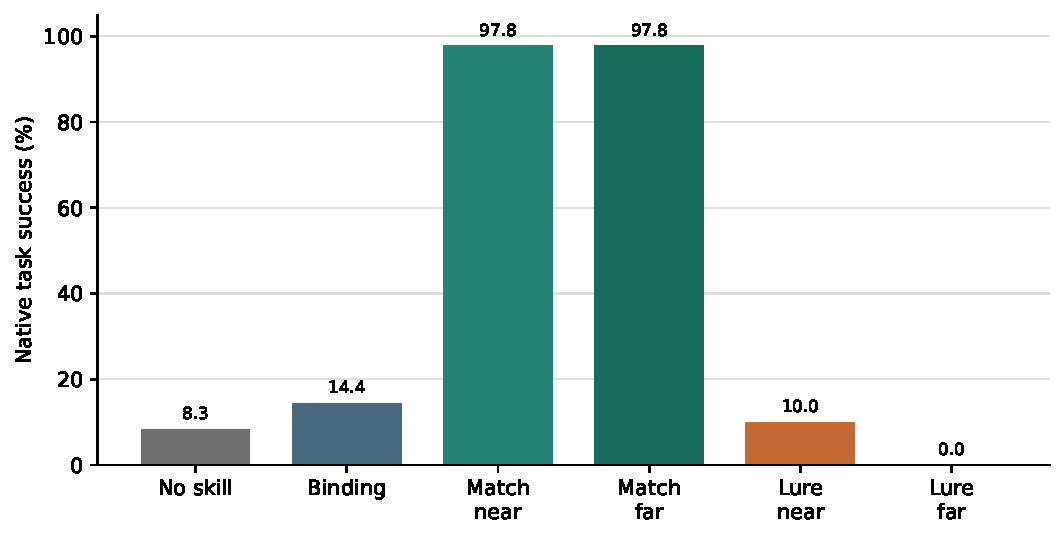
\includegraphics[width=0.82\linewidth]{condition_success.pdf}}{}
\caption{六个冻结条件下的原生成功率。条件之间只改变来源程序与词面排序，同一
目标--模型块从完全相同的原生状态开始。}
\label{fig:success}
\end{figure}

\subsection{执行器帮助之外的因果贡献}
仅绑定条件成功率为 \BindingRate\%。相对这个共享非程序守卫的公平对照，匹配
远来源产生 \HelpfulCount{} 个有帮助差异和 \HarmfulCount{} 个有害差异，净
因果效应为 \CausalNet{} 点，伤害率为 \HarmRate\%。该比较比“匹配远与无
Skill”更严格，因为两侧具有完全相同的目标绑定、错误对象拒绝、候选限制和
循环抑制。

\subsection{异质性与失败边界}
\IfFileExists{../../results/confirmation/analysis/table_by_model_zh.tex}{
\begin{table}[t]
\centering
\caption{各模型的主效应（匹配远减诱饵近）。}
\label{tab:model}
\begin{tabular}{lr}
\toprule
模型 & 效应（百分点） \\
\midrule
Qwen3-4B & 88.3 \\
Phi-4-mini & 88.3 \\
Mistral-7B-v0.3 & 86.7 \\
\bottomrule
\end{tabular}
\end{table}
}{}
\IfFileExists{../../results/confirmation/analysis/table_by_family_zh.tex}{
\begin{table}[t]
\centering
\caption{各 ALFWorld 原生任务族的主效应。}
\label{tab:family}
\begin{tabular}{lr}
\toprule
任务族 & 效应（百分点） \\
\midrule
简单放置 & 33.3 \\
清洗后放置 & 100.0 \\
加热后放置 & 100.0 \\
冷却后放置 & 100.0 \\
灯下查看 & 100.0 \\
双对象放置 & 93.0 \\
\bottomrule
\end{tabular}
\end{table}
}{}

冻结规则要求多个模型与任务族上的主效应为正。分任务族报告尤其重要：错误的
数量契约仍可能碰巧完成单对象单调目标，而单对象诱饵会在双对象目标完成前确定
停止；转换诱饵可能因设备不存在而失败。相反，匹配契约也可能因为探索耗尽步数
而失败。CSTT 保留全部结果，因为它测试兼容性的行为后果，而不预设兼容一定
成功。

\subsection{审计与成本}
每个模型运行只有在独立日志审计通过后才被接收。审计检查每臂唯一记录、块内
初始状态哈希、所有选择动作均来自原生菜单、候选/拒绝划分完整、来源分配有效，
并确认运行输入没有目标金标准计划。完成记录包含墙钟时间、CUDA 峰值分配和
Episode 文件哈希；每个条件的 Token 与步数总量也随结果发布，便于同时比较
迁移收益与交互成本。

\section{讨论}
CSTT 把问题从“Agent 带 Skill 是否成功”改为“来源资产的哪一部分改变了同一
目标的结果”。交叉设计提供三类部署信号：匹配与诱饵差大，支持程序感知选择；
匹配与仅绑定差小，说明收益主要来自目标落地或搜索守卫；伤害率高，则技能库即使
平均成功率提高也应考虑弃权。

研究也说明相似度为什么不是完整检索目标。词面重叠能够提示实体和主题，却不能
表示对象数量、必要转换、终止条件和资源顺序。这不表示语义相似度无用；实际
检索器应把它与兼容性表示结合，并用 CSTT 一类测试同时验证二者。

有限状态执行器是实验仪器，不是本文声称的最终 Agent 架构。它的作用是在两个
提示机制失败后，让来源程序的干预具体且可审计。生产系统可以通过规划、约束
解码、代码或工具实现契约；只要六种条件能够重置并记录，CSTT 仍可使用。

\section{有效性威胁}
\paragraph{构念有效性。}
ALFWorld 任务族具有较清晰的程序签名。当前契约捕捉数量、一个转换和最终放置，
不能覆盖丰富自然语言语义。原生奖励证明任务完成，但不包含安全性和可取行为的
全部维度。

\paragraph{内部有效性。}
仅绑定对照共享非程序守卫，六臂共享精确初始状态，但候选动作约束可能与不同
模型发生不同交互。因此本文分开报告执行器效应与 Skill 因果效应，并披露全部
模型。来源选择是确定且结果盲的；冻结哈希能防止事后修改，但不是对所有基础设施
故障的形式化证明。

\paragraph{外部有效性。}
确认覆盖一个具身文本环境、六个任务族、三个中小型开放模型，而且大多数目标
来自 ALFWorld `valid\_seen`。仅有一个 `valid\_unseen` 目标，不足以提出单独的
未见环境泛化结论。本文的“未参与”主要指与开发和前序论文证据零重叠，不代表
开放技能市场的总体样本。还需要跨环境、Web、API、多 Agent 和闭源模型复现。

\paragraph{统计有效性。}
目标是抽样聚类单位；严格排除既有证据耗尽了若干任务族，因此配额不均衡。本文
同时强制微平均与六族等权宏平均。置信区间表示对当前名单中目标重抽样的不确定
性，不表示所有编译器和环境上的不确定性。

\section{复现与责任边界}
发布目录包含冻结配置和哈希、目标/来源配对、全部 Episode 日志、独立审计、
配对分析记录、测试、中英文源码与 PDF，以及校验清单。发布记录验证只需 CPU；
完整原生复现需要一张 24 GB 显卡。来源演示和目标游戏遵守 ALFWorld 的再发布
条款。研究只评估良性程序复用，不增加攻击能力。

本文不声称词面相似度普遍有害，不声称每个兼容 Skill 都改善每个目标，不声称
CSTT 能检索最佳 Skill，也不把 ALFWorld 实例级证据解释为跨域迁移。得到支持
的结论更窄：在冻结的编译器和执行器下，同状态交叉检验能够把可靠目标收益归因
到程序兼容性，而不是词语重叠或非程序执行辅助。

\section{结论}
可复用 Skill 的评测需要反事实，而不只是成功计数。CSTT 使用真实成功来源交叉
程序兼容性与词面相似度，加入无 Skill 和公平仅绑定对照，并在同一原生状态上
执行六个条件。冻结确认回答三个实际问题：词面远但兼容的程序能否优于词面近的
错误诱饵；收益能否在扣除执行器帮助后保留；结论的边界在哪里。由此，技能迁移
证据可以服务于技能库选择、发布门禁和生命周期维护，而不会把一个评测协议夸大
为普遍迁移能力。

\bibliographystyle{plainnat}
\bibliography{../references}

\end{document}
